

\begin{frame}{\ft{Using Custom Viewers}}

\doubleFrame{Re-PDF data is delivered to potential 
buyers embedded in PDF files so that buyers can open 
these files even if they do not have the Re-PDF software.  
As a result, users will not be burdened with files that 
they cannot open or identify.  At the same time, 
users that \textit{do} install the Re-PDF viewer will 
experience the Re-PDF presentations interactively --- adding 
many layers to the ordinary PDF experience.}

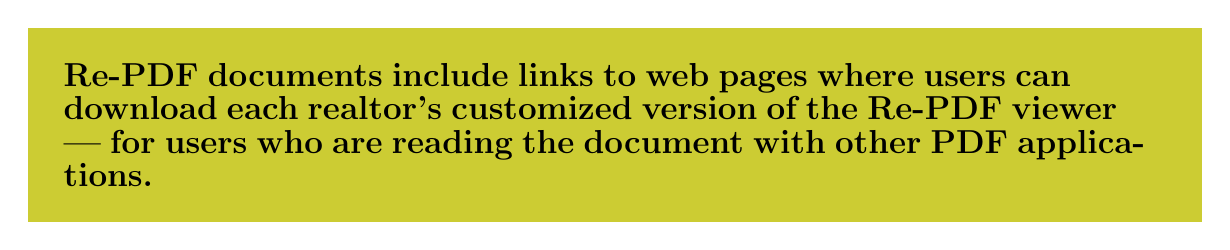
\begin{tikzpicture}
%\nodeincludegraphics[0.88\textwidth]{screenshots/ss-norpdf.png}
\nodeincludegraphicsTR{2.5cm}{2cm}{screenshots/ss-norpdf.png}

\ann{darkRed}{0.7}{1mm}{grammarArrowColor}{0.5}{6,3.5}{6.5}{1}{0.85}
%\node [anchor=west] (note) at (-1,3) {\Large Note};
%\draw [-latex, ultra thick, red] (note) to[out=0, in=-120] (0.48,0.80);

 \node [anchor=west,fill=blue!20!yellow,inner sep=13, text width=14cm]
  (longnote) at (1.5,1.5) {%  %{\color{rb!85!red}{
  {\cframedboxyellow{\large \textbf{Re-PDF documents include links 
  to web pages where users can download each 
  realtor's customized version of the Re-PDF viewer 
  --- for users who are reading the 
  document with other PDF applications.}}}};


\end{tikzpicture}


\end{frame}

